% cube solid-geometry section figure (Liaoning 2008 q19), oblique projection
% 3D (x,y,z) -> 2D (4x+1.3y, 3.5z+1.2y), b=1/2 generic position
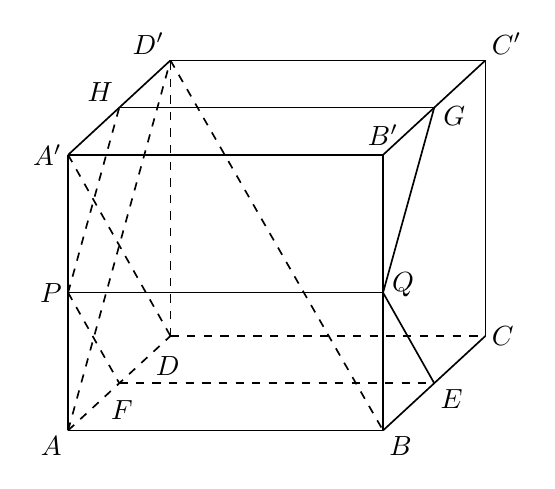
\begin{tikzpicture}[x=1cm,y=1cm,line width=.6pt,font=\normalsize,
  cube edge/.style={solid,line width=.6pt},
  cube hidden/.style={dashed,line width=.6pt},
  cube label/.style={font=\normalsize,inner sep=2pt}]
\coordinate (A) at (0,0);
\coordinate (B) at (4,0);
\coordinate (Bp) at (4,3.5);
\coordinate (Ap) at (0,3.5);
\coordinate (D) at (1.3,1.2);
\coordinate (C) at (5.3,1.2);
\coordinate (Cp) at (5.3,4.7);
\coordinate (Dp) at (1.3,4.7);
\coordinate (P) at (0,1.75);
\coordinate (Q) at (4,1.75);
\coordinate (F) at (0.65,0.6);
\coordinate (E) at (4.65,0.6);
\coordinate (H) at (0.65,4.1);
\coordinate (G) at (4.65,4.1);
% --- solid cube edges ---
\draw[cube edge] (A)--(B);
\draw[cube edge] (A)--(P)--(Ap);
\draw[cube edge] (B)--(Q)--(Bp);
\draw[cube edge] (Ap)--(Bp);
\draw[cube edge] (B)--(E)--(C);
\draw[cube edge] (C)--(Cp);
\draw[cube edge] (Dp)--(Cp);
\draw[cube edge] (Ap)--(H)--(Dp);
\draw[cube edge] (Bp)--(G)--(Cp);
% --- solid section edges ---
\draw[cube edge] (P)--(Q);
\draw[cube edge] (Q)--(E);
\draw[cube edge] (Q)--(G);
\draw[cube edge] (G)--(H);
% --- dashed cube edges ---
\draw[cube hidden] (D)--(C);
\draw[cube hidden] (D)--(Dp);
\draw[cube hidden] (A)--(F)--(D);
% --- dashed section edges ---
\draw[cube hidden] (F)--(E);
\draw[cube hidden] (P)--(F);
\draw[cube hidden] (P)--(H);
% --- reference diagonals present in original ---
\draw[cube hidden] (A)--(Dp);
\draw[cube hidden] (Ap)--(D);
\draw[cube hidden] (Dp)--(B);
% --- labels (offset to avoid lines) ---
\node[cube label,below left] at (A) {$A$};
\node[cube label,below right] at (B) {$B$};
\node[cube label,left] at (Ap) {$A'$};
\node[cube label,above,yshift=1pt] at (Bp) {$B'$};
\node[cube label,above left] at (Dp) {$D'$};
\node[cube label,above right] at (Cp) {$C'$};
\node[cube label,right] at (C) {$C$};
\node[cube label,below,yshift=-5pt,xshift=-1pt] at (D) {$D$};
\node[cube label,left] at (P) {$P$};
\node[cube label,right,xshift=1pt,yshift=3pt] at (Q) {$Q$};
\node[cube label,below,yshift=-4pt,xshift=1pt] at (F) {$F$};
\node[cube label,below right] at (E) {$E$};
\node[cube label,above left] at (H) {$H$};
\node[cube label,right,xshift=1pt,yshift=-3pt] at (G) {$G$};
\end{tikzpicture}
